\fancychapter{Simulations}
\label{chap:sims}

    Simulations were used to validate the converter design and the \ac{mppt} algorithm before hardware implementation. This chapter presents LTspice simulations of the photovoltaic model and the boost converter, an analytical power-loss estimate in MATLAB, and the evaluation of the tracking algorithm in Simulink.

    \section{DC-DC converter}

        The converter was simulated in LTspice to confirm the component selection under representative charging conditions. This section presents the photovoltaic cell model and the boost converter simulations used to compare inductor and capacitor options and to estimate ripple and efficiency.

    \subsection{Solar panel model}

        The simulations started in LTspice to test the converter under different conditions. To achieve that, a \ac{pv} electrical model of the cells was designed using a five parameter model (1M5P) configuration. More electrical models can simulate a solar panel, some with higher accuracy but greater complexity. This model was ideal for the simulation because it is both reliable and simple.

        The 1M5P model represents the solar cell as a single-diode equivalent circuit with a current source, a diode, a series resistance $R_s$ and a shunt resistance $R_{sh}$, as shown in Figure~\ref{fig:pv_model}. The current source models the photogenerated current $I_{ph}$, the diode the nonlinear $I$-$V$ characteristic of the p-n junction, $R_s$ the ohmic losses in the material and contacts, and $R_{sh}$ the leakage current.

        The output current is given by Equation~\ref{eq:1m5p}, where $I_0$ is the diode saturation current, $n$ the ideality factor and $V_t$ the thermal voltage \cite{LOBRANO2013894}. Together with $I_{ph}$, $R_s$ and $R_{sh}$, these five parameters give the model its name.

        \begin{equation}
            I = I_{ph} - I_0 \left[ \exp\left(\frac{V + I R_s}{n V_t}\right) - 1 \right] - \frac{V + I R_s}{R_{sh}}
            \label{eq:1m5p}
        \end{equation}

        These parameters are not directly provided by manufacturers, but can be extracted from the standard datasheet values, namely the open-circuit voltage ($V_{oc}$), short-circuit current ($I_{sc}$), voltage and current at the \ac{mpp} ($V_{mp}$, $I_{mp}$), and the respective temperature coefficients, through a set of equations that ensure the model matches these reference points under \ac{stc}. There are several ways to do it, however, it is outside the range of this work. To simplify, it was used an online tool for the calculations, which we will not explain in detail here. 

        \begin{figure}[!ht]
            \centering
            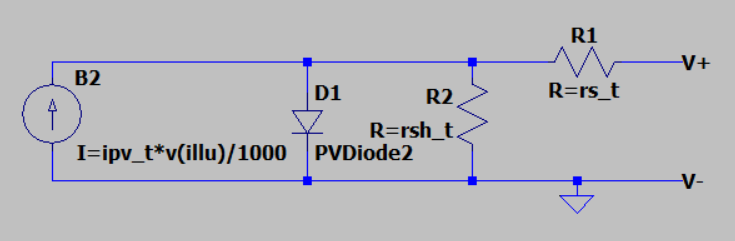
\includegraphics[width=0.6\textwidth]{Images/Implementation/PV model.png}
            \caption{Solar panel model diagram (1M5P configuration).}
            \label{fig:pv_model}
        \end{figure}
        
    \subsection{Boost converter}
    \label{subsubsect:Sim_Boost}
        To validate the theoretical calculations, simulations in LTspice were carried out using the boost converter in steady state mode and a fixed duty cycle. 

        Considering a solar panel operating at its \ac{mpp} with 35 cells, five points of the CC-CV charging curve were chosen to test the performance of the converter. Figure~\ref{fig:cc-cv points} shows these five points.
        
        \begin{figure}[!ht]
            \centering
            % 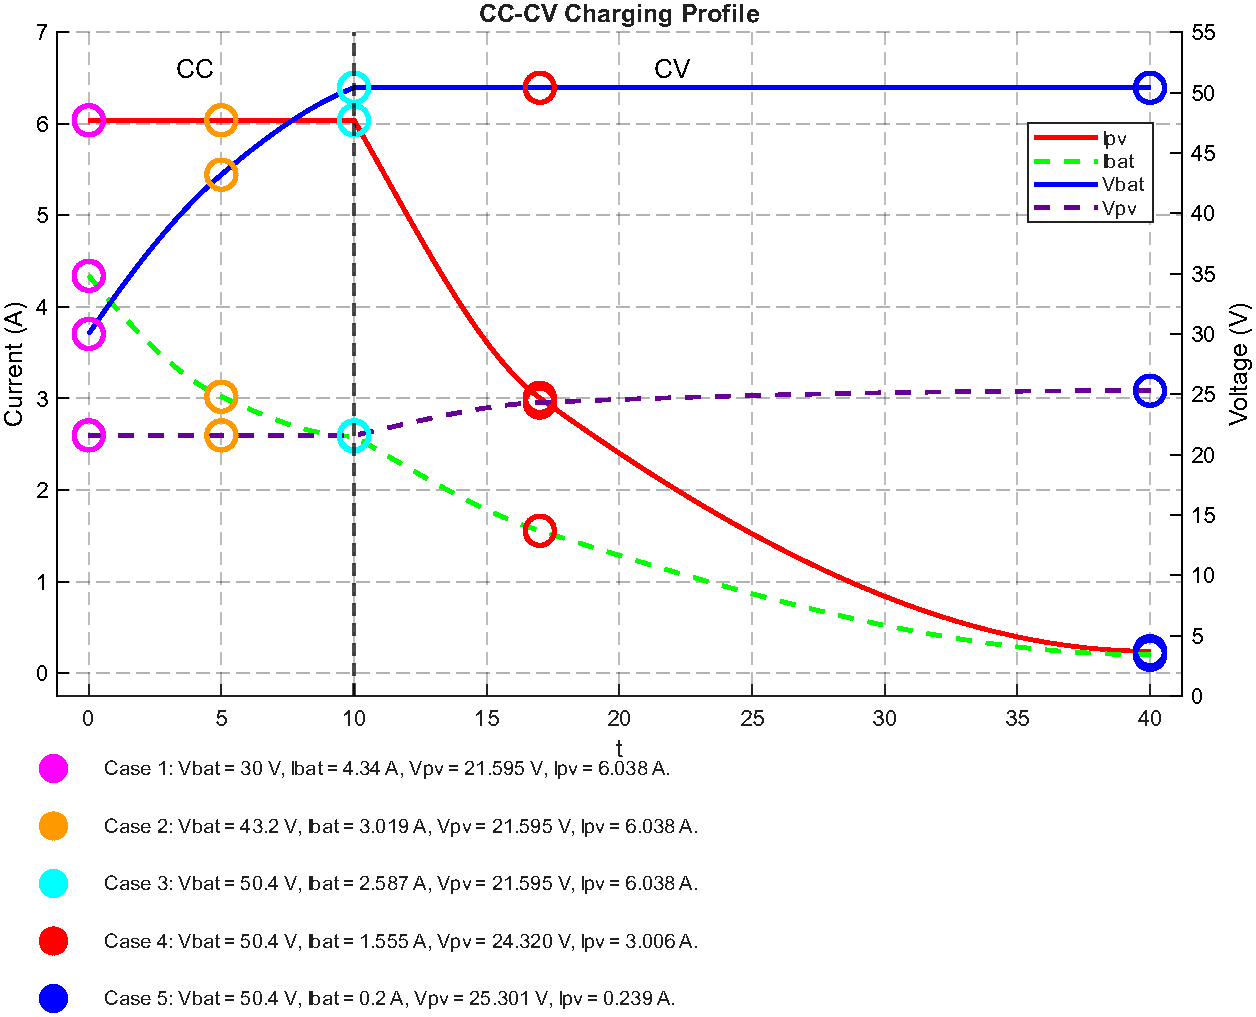
\includegraphics[width=0.7\textwidth]{Images/Implementation/cc_cv_points.pdf}
            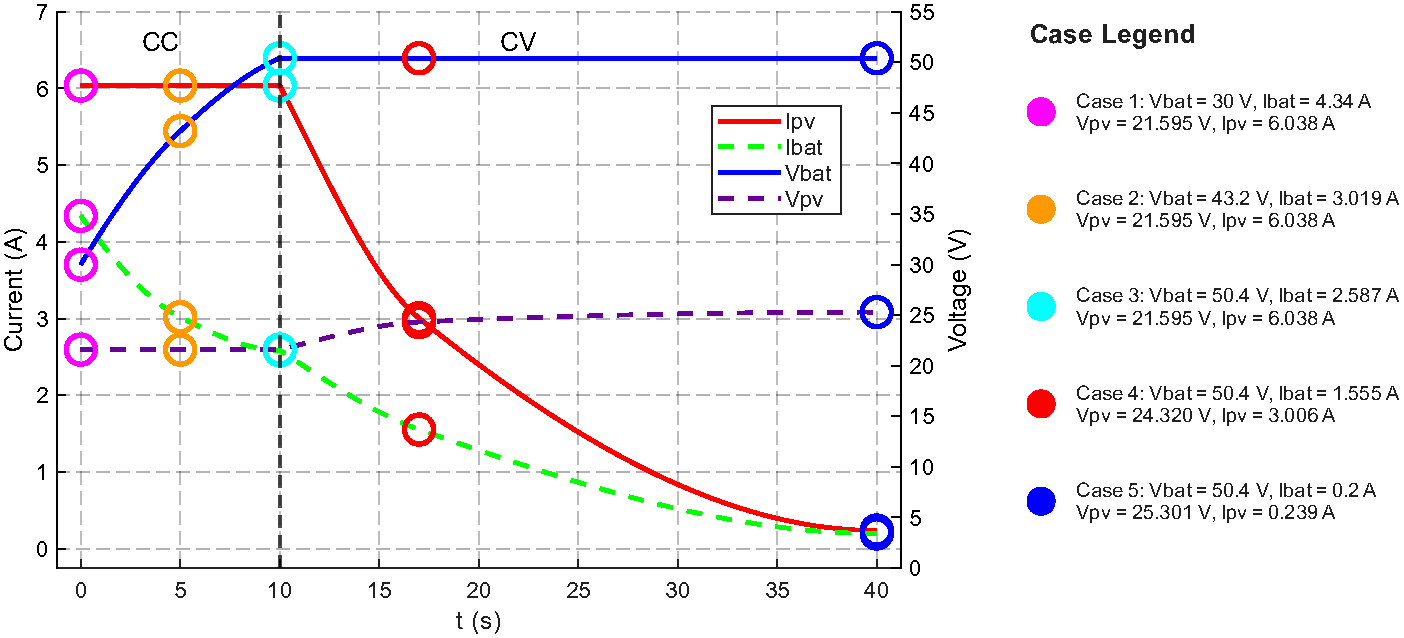
\includegraphics[width=0.8\textwidth]{Images/Implementation/cc_cv_points_right.pdf}
            \caption{Draft of CC-CV charge characteristics and analysis point selection.}
            \label{fig:cc-cv points}
        \end{figure}

        It is important to note that, in this \ac{cc}-\ac{cv} charging profile, the constant current is determined by the solar panel rather than the battery, as is typically assumed. This is only possible because the maximum charging current of the battery is lower than the maximum current that can be supplied by the solar panel. Therefore, during the \ac{cc} phase, the converter operates at the \ac{mpp} of the solar panel.

        The timescale of the charging process also depends on the battery capacity, with larger capacities requiring longer charging times under otherwise equivalent conditions.


        With the chosen five points, some simulations were carried out using capacitors and inductors that would fit the requirements calculated earlier. The objective of these simulations is to optimize the performance of the converter, leading to better choices.

        The model was built in LTspice using manufacturer component models, except for the solar panel, which was implemented as described above. The battery was represented by a voltage source and a series resistor, and the transistor dead time was set to the prototype value, using the measured rise and fall times. Figure~\ref{fig:sim_circuit} shows the simulation circuit and his parameters.

        \begin{figure}[!ht]
            \centering
            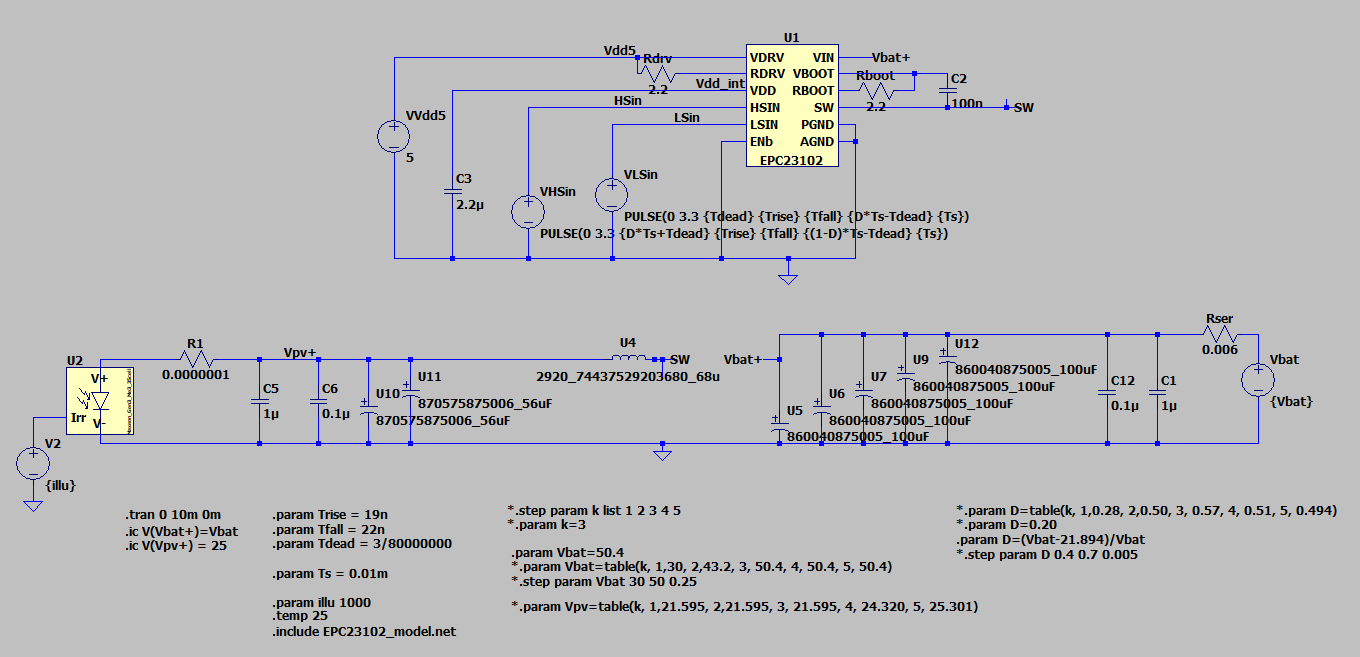
\includegraphics[width=0.70\textwidth]{Images/Implementation/Sim_circuit.png}
            \caption{Simulation circuit schematic.}
            \label{fig:sim_circuit}
        \end{figure}


        The first simulations were carried out to choose the input and output capacitors. The idea is to simulate the circuit using a known inductor ($68~\mu\mathrm{H}$) and change the capacitors for different configurations. All configurations are overdimensioned to give low ripples (current and voltage). So the main factor is the efficiency of the converter.

        Table~\ref{tab:loss_capacitors_2} shows the results. The efficiency of all combinations is very high, however, the highest is the one with two $56~\mu\mathrm{F}$ as input capacitors and three $220~\mu\mathrm{F}$ capacitors as output capacitors. Unfortunately, the $220~\mu\mathrm{F}$ capacitors were not available at the time, so the second best option was chosen: five $100~\mu\mathrm{F}$ capacitors.

        It is worth noting that this is a simulation and therefore the efficiency is higher than what will be measured in laboratory results. Additionally, the difference between each combination is very small. To make the product cheaper, the third option would be as good as the one chosen.

        
        \begin{table}[!ht]
            \caption{Loss (\%) for different capacitor configurations (Cin, Cout).}
            \centering
            \begin{tabular}{|c|cccc|}
            \hline
            \textbf{Case \#} & \textbf{$2\times56~\mu\mathrm{F}$, $3\times220~\mu\mathrm{F}$} & \textbf{$100~\mu\mathrm{F}$, $3\times220~\mu\mathrm{F}$} & \textbf{$100~\mu\mathrm{F}$, $5\times100~\mu\mathrm{F}$} & \textbf{$2\times56~\mu\mathrm{F}$, $5\times100~\mu\mathrm{F}$} \\
            \hline
            1 & 0.5729 & 0.5796 & 0.5856 & 0.5788 \\
            2 & 0.6762 & 0.6985 & 0.7069 & 0.6844 \\
            3 & 0.7359 & 0.7655 & 0.7743 & 0.7449 \\
            4 & 0.6654 & 0.7091 & 0.7161 & 0.6735 \\
            5 & 3.4177 & 3.7148 & 3.7554 & 3.4671 \\
            \hline
            \end{tabular}
            
            \label{tab:loss_capacitors_2}
        \end{table}

        As in the previous simulation, the inductor was chosen by keeping all components with the same values (the capacitors used were $C_\mathrm{in} = 2\times56~\mu\mathrm{F}$ and $C_\mathrm{out} = 5\times100~\mu\mathrm{F}$) and changing the inductor. Similar to before, all inductors simulated are within the minimum required.

        Table~\ref{tab:loss_inductance_2} shows the losses and the inductor current ripple for each charging case. As before, the efficiency difference is very low but less linear than in the previous simulation, likely due to the inductor models chosen. The chosen inductor strongly influences the input ripple, which can generate heat and electrical interference. The $22~\mu\mathrm{H}$ inductor showed a higher ripple current, reaching values close to the input current. The inductor chosen was $68~\mu\mathrm{H}$, since it has overall good efficiency and a reasonable inductor current ripple.

        \begin{table}[!ht]
            \caption{Loss (\%) and $\Delta i_{L}$ ($I_{L,\max}-I_{L,\min}$) for different inductance values.}
            \centering
            \small
            \setlength{\tabcolsep}{4pt}
            \begin{tabular}{|c|ccccc|ccccc|}
            \hline
            \multirow{2}{*}{\textbf{Case \#}} & \multicolumn{5}{c|}{\textbf{Loss (\%)}} & \multicolumn{5}{c|}{\textbf{$\Delta i_{L}$ (A)}} \\
            \cline{2-11}
            & \textbf{$22~\mu\mathrm{H}$} & \textbf{$33~\mu\mathrm{H}$} & \textbf{$47~\mu\mathrm{H}$} & \textbf{$68~\mu\mathrm{H}$} & \textbf{$100~\mu\mathrm{H}$}
            & \textbf{$22~\mu\mathrm{H}$} & \textbf{$33~\mu\mathrm{H}$} & \textbf{$47~\mu\mathrm{H}$} & \textbf{$68~\mu\mathrm{H}$} & \textbf{$100~\mu\mathrm{H}$} \\
            \hline
            1 & 0.4206 & 0.4439 & 0.5453 & 0.5788 & 1.2659 & 2.6939 & 1.8906 & 1.3256 & 0.9781 & 0.6251 \\
            2 & 0.6645 & 0.6793 & 0.6627 & 0.6844 & 1.3664 & 4.7934 & 3.3416 & 2.3354 & 1.7066 & 1.0707 \\
            3 & 0.7883 & 0.8076 & 0.7290 & 0.7449 & 1.4193 & 5.4733 & 3.8253 & 2.6813 & 1.9644 & 1.2839 \\
            4 & 1.0556 & 1.0583 & 0.6867 & 0.6735 & 0.9624 & 5.5596 & 3.8565 & 2.7075 & 2.0139 & 1.2925 \\
            5 & 6.7045 & 6.6230 & 3.6556 & 3.4671 & 3.8177 & 5.5520 & 3.8510 & 2.6903 & 1.9636 & 1.2344 \\
            \hline
            \end{tabular}
            \label{tab:loss_inductance_2}
            \label{tab:delta_iin_inductance}
        \end{table}

        Now that the converter components are all chosen, the following measurements were taken in LTspice (Table~\ref{tab:ripple_loss}).

        \begin{table}[!ht]
        \centering
        \caption{Ripple and power loss summary for each operating point.}
        \label{tab:ripple_loss}
        \begin{tabular}{|c|cccc|}
        \hline
        \textbf{Case \#} & \textbf{$\Delta V_{bat}$ (V)} & \textbf{$\Delta V_{pv}$ (V)} & \textbf{$\Delta I_{L}$ (A)} & \textbf{Loss (\%)} \\
        \hline
        1 & 0.0406 & 0.0145 & 0.9781 & 0.578 \\
        2 & 0.0491 & 0.0212 & 1.7066 & 0.684 \\
        3 & 0.0529 & 0.0244 & 1.9644 & 0.745 \\
        4 & 0.0406 & 0.0220 & 2.0139 & 0.674 \\
        5 & 0.0302 & 0.0215 & 1.9636 & 3.464 \\
        \hline
        \end{tabular}
        \end{table}


        Both voltage ripples are lower than the goal defined in Table~\ref{tab:converter_constraints}. As for the current ripple, it is still reasonable. The losses/efficiency are also higher than what was aimed for, reaching efficiency values up to 99.4\%. 

        A voltage sweep was performed, and as expected, the efficiency drops with the increase of output voltage (Figure~\ref{fig:voltage_sweep}). Also, as mentioned earlier, the output current drops because, in \ac{cc} mode, the solar panel current is constant, so the output current decreases as battery voltage increases due to power conservation.

        \begin{figure}[!ht]
            \centering
            \begin{subfigure}{0.49\textwidth}
                \centering
                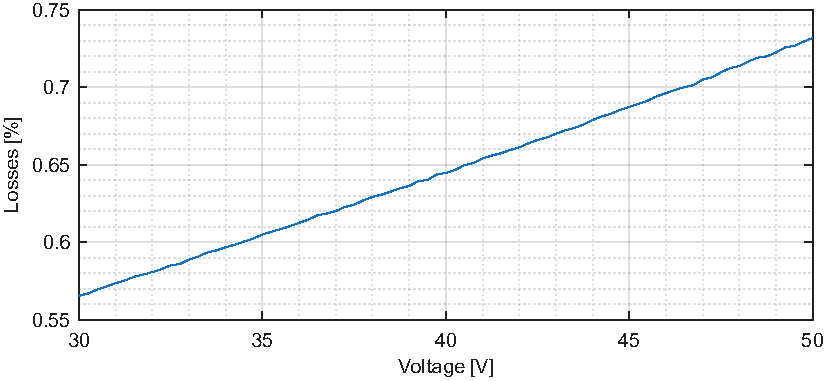
\includegraphics[width=0.99\textwidth]{Images/Implementation/vbat__sweep_sim_res.pdf}
                \caption{Losses (\%) over battery voltage.}
            \end{subfigure}
            \hfill
            \begin{subfigure}{0.49\textwidth}
                \centering
                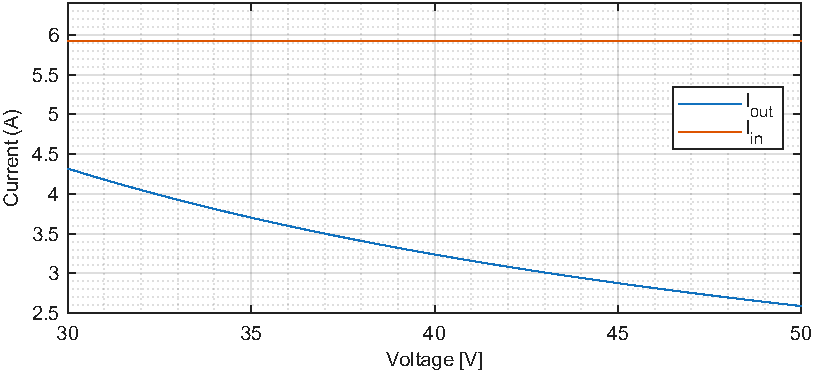
\includegraphics[width=0.99\textwidth]{Images/Implementation/vbat__sweep_sim_res2.pdf}
                \caption{Output and input current over battery voltage.}
            \end{subfigure}
            \caption{Battery voltage sweep simulation results (solar panel in \ac{mpp}).}
            \label{fig:voltage_sweep}
        \end{figure}

        % \begin{figure}[!ht]
        %     \centering
        %     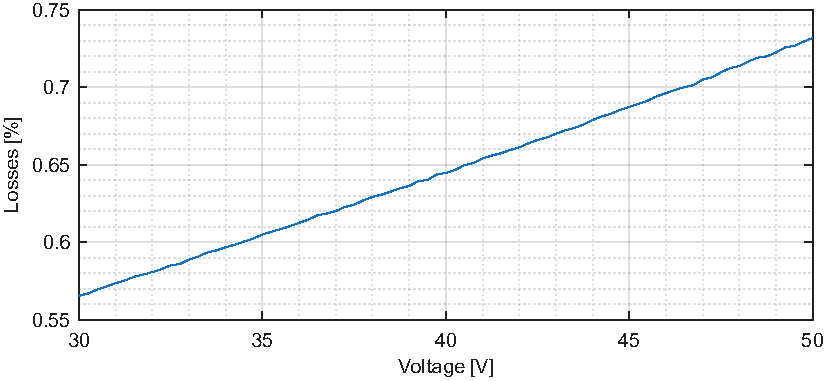
\includegraphics[width=0.7\textwidth]{Images/Implementation/vbat__sweep_sim_res.pdf}
        %     \caption{Battery voltage sweep simulation results.}
        %     \label{fig:voltage_sweep}
        % \end{figure}

        Note: two Schottky diodes added in prototype version 1.1 were not included in these simulations. They increase the simulated efficiency by only $+0.03\%$, which is negligible given the short dead time ($0.375\%$ of the PWM period).

    \section{Power loss estimation}
        \label{subsubsec:loss_estimation}

        Although LTspice provides an accurate estimate of converter efficiency, it does not directly identify each component's contribution to total power dissipation. Therefore, an analytical power loss estimation was developed in MATLAB to estimate the individual losses of each component of the designed synchronous boost converter. This estimation uses the electrical parameters of the selected components from their datasheets, along with the converter operating conditions.

        The total prototype losses are obtained by summing the losses associated with the GaN transistors, inductor, capacitors and auxiliary electronics:

        \begin{equation}
        P_{loss}=P_{tran}+P_{L}+P_{C}+P_{aux}.
        \end{equation}

        The prototype efficiency is then calculated as:

        \begin{equation}
        \eta=\frac{P_{out}}{P_{out}+P_{loss}}\times100\%.
        \end{equation}

        The transistor losses can be split in three. The conduction, switching and deadtime losses:
        \begin{equation}
            P_{tran}=P_{cond_{HS}}+P_{cond_{LS}}+P_{sw_{HS}}+P_{sw_{LS}}+P_{dead}
        \end{equation}

        The conduction losses of each GaN transistor are given by:

        \begin{equation}
        P_{cond}=I_{RMS}^{2}R_{DS(on)}.
        \end{equation}

        These losses are primarily caused by the on state resistance of the transistors, resulting in power dissipation whenever current flows through the transistors. 

        The switching losses are estimated using Equation~\ref{eq:psw}, 
        which takes into account the losses during the period when the transistor is neither fully on nor fully off. They also include the losses associated with charging and discharging the output capacitance of each transistor.

        \begin{equation}
        P_{sw}=\frac{1}{2}V_{out}I_{L_{AVG}}(t_r+t_f)f_{sw} + \frac{1}{2}C_{oss}V_{out}^{2}f_{sw}
        \label{eq:psw}
        \end{equation}

        The deadtime losses are calculated using Equation~\ref{eq:pdead}. These losses originate from the conduction of the reverse conduction path during the dead time interval required to prevent shoot through. This reverse conduction path is either from the third-quadrant conduction of the GaN device or from the parallel Schottky diode added later in version 1.1 of the prototype.

        \begin{equation}
        P_{dead}=2\cdot  V_f \cdot I_{L_{AVG}} \cdot t_{dead} \cdot f_{sw}.
        \label{eq:pdead}
        \end{equation}

        The inductor and \acs{dc} capacitor losses are estimated using the RMS current passing through them and their \ac{esr}. The inductor manufacturer does not provide the required magnetic material parameters to estimate the \acs{ac} losses. However, an employee suggested using their own tool called REDEXPERT, which can simulate both \acs{dc} and \acs{ac} losses. Therefore, the value \acs{ac} losses were copied from their tool

        \begin{equation}
        P_L=I_{L_{RMS}}^{2}ESR + P_{L_{AC}}.
        \end{equation}

        \begin{equation}
        P_C=I_{C_{RMS}}^{2}ESR,
        \end{equation}

        

        The gate driver losses are estimated using Equation~\ref{eq:gate_drive} which takes into account the energy needed to drive the transistors. Although the EPC23102 has an internal gate driver, this is still relevant.

        \begin{equation}
        P_{gate}= (Qg_{LS} + Qg_{HS})* Vdrv * fsw.
        \label{eq:gate_drive}
        \end{equation}

        Last but not least, the rest of the electronics (\acs{mcu}, \acs{dc}-\acs{dc}, sensors, etc.) were considered too. The sum of the maximum currents of all components was calculated. Then the power losses was estimated based on the power and efficiency of each \acs{dc}-\acs{dc} converter, Equation~\ref{eq:aux_losses}.

        \begin{equation}
            P_{aux} = (I_{3v3} * 3.3) * eff_{dcdc} + (I_{5} * 5) * eff_{dcdc} + I_{in}*R_{shunt} + I_{out}*R_{shunt} + P_{gate}
            \label{eq:aux_losses}
        \end{equation}

        Figure~\ref{fig:loss_breakdown} shows the resulting power-loss distribution. The calculated total power loss is approximately 1.98~W, corresponding to 98.50\% efficiency. This is about $1\%$ lower than the LTspice result, and a further reduction is expected in the laboratory because \ac{pcb} parasitics were not included.

        \begin{figure}[!ht]
            \centering
            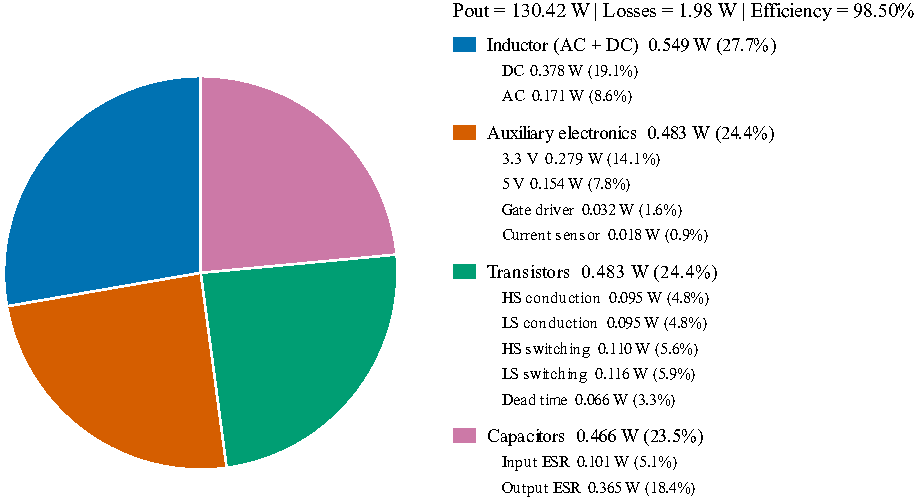
\includegraphics[width=0.55\textwidth]{Images/Implementation/fig_loss_breakdown.pdf}
            \caption{Prototype analytical power loss distribution at Case~2.}
            \label{fig:loss_breakdown}
        \end{figure}

        The inductor \acs{dc} losses are the largest term, followed by the auxiliary electronics (mainly the auxiliary \acs{dc}--\acs{dc} conversion), the GaN transistor losses ($24.4\%$) and the capacitors ($23.5\%$). Overall, nearly half of the losses come from passive components and about one quarter from the semiconductors. Despite this, both the simulation and the analytical model indicate a highly efficient converter.



    \section{MPPT algorithm}
        The algorithm parameters (switching and sampling frequencies, step size and power dead band) must be tuned for speed without compromising stability. A MATLAB Simulink model of the boost converter, solar panel and battery was therefore used to evaluate the tracker (Figure~\ref{fig:Simulink mode}). A diode replaces the synchronous high-side switch, which does not affect the algorithm comparison.

        \begin{figure}[!ht]
            \centering
            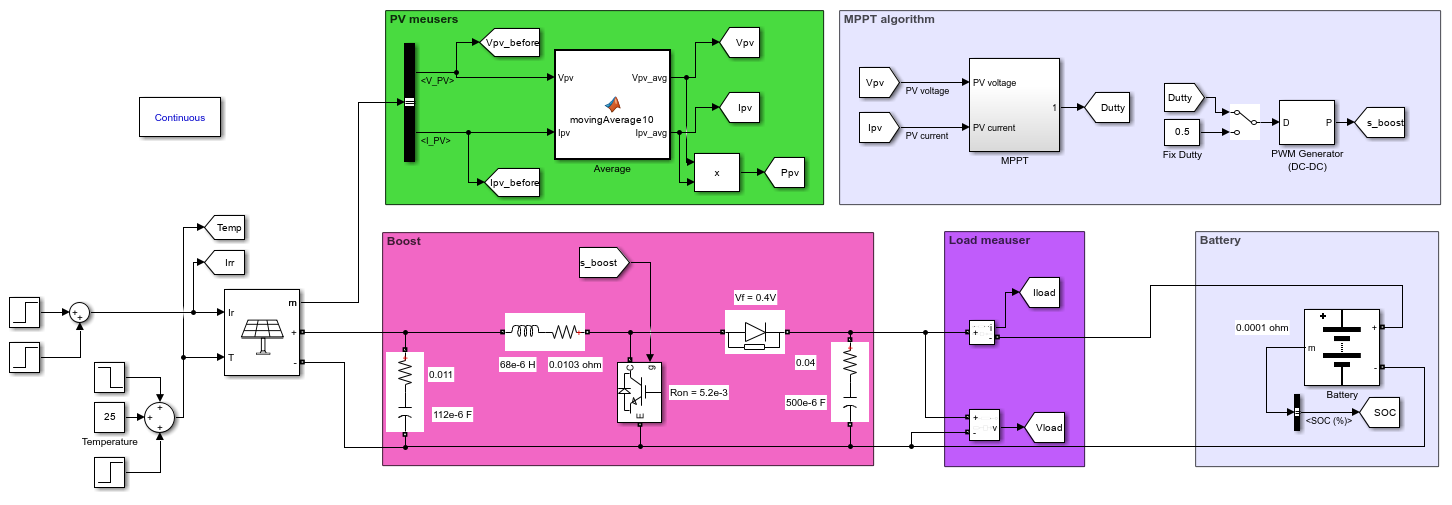
\includegraphics[width=0.75\textwidth]{Images/Implementation/simulink_sim.png}
            \caption{MATLAB Simulink MPPT simulation model.}
            \label{fig:Simulink mode}
        \end{figure}

        The panel (35 cells) and the \ac{sg01} battery match the real system. Measurement noise is included on the \ac{pv} side and averaged over 10 samples at $1~\mathrm{kHz}$ before being sent to the algorithm, which runs at $100~\mathrm{Hz}$ and implements both the sweep and \ac{peo}.

        To understand the impact of each environment variation on the \ac{mpp} point, a sweep  was performed for different irradiance values and temperatures (Figures~\ref {fig:irr_sweep} and \ref{fig:temp_sweep}). For irradiance variations, the maximum duty cycle difference is 3\%. In contrast, the maximum duty cycle difference for temperature variations is 9\%. This means the algorithm will always be slower to temperature variations than to irradiance variations. However, it is more common to have a fast changing irradiance than temperature. The solar panels will heat slowly, and when covered in water, they cool by around $10~^\circ\mathrm{C}$ to $20~^\circ\mathrm{C}$ (values measured during tests).  

        \begin{figure}[!ht]
            \centering
            \begin{minipage}[b]{0.49\textwidth}
                \centering
                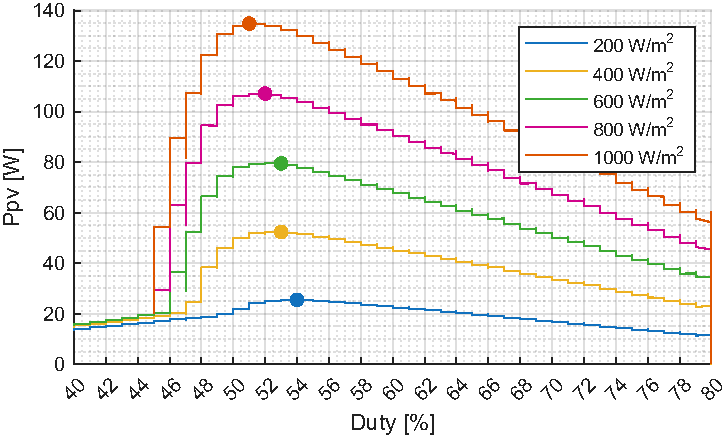
\includegraphics[width=\textwidth]{Images/LAB_res/sweep_duty_irr.pdf}
                \caption{Duty cycle sweep with different values of irradiance.}
                \label{fig:irr_sweep}
            \end{minipage}
            \hfill
            \begin{minipage}[b]{0.49\textwidth}
                \centering
                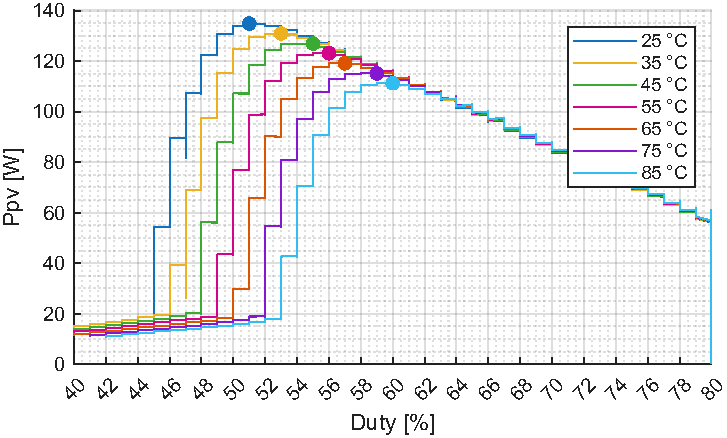
\includegraphics[width=\textwidth]{Images/LAB_res/sweep_duty_temp.pdf}
                \caption{Duty cycle sweep with different values of temperature.}
                \label{fig:temp_sweep}
            \end{minipage}
        \end{figure}

        In the worst case ($9\%$), a tracking time of $0.5~\mathrm{s}$ at $100~\mathrm{Hz}$ allows 50 steps, i.e.\ an ideal step of $0.18\%$. Such a small step is easily confused with noise, so the parameters must be tuned to the actual system.

        With the frequency fixed at $100~\mathrm{Hz}$, three step sizes were compared under successive temperature steps (Figure~\ref{fig:peo_step_comparison}). The smallest step never reaches the \ac{mpp}, most likely because of noise. The other two perform similarly, but the larger step oscillates more around the \ac{mpp}.


        \begin{figure}[!ht]
            \centering

            \begin{subfigure}[b]{0.49\textwidth}
                \centering
                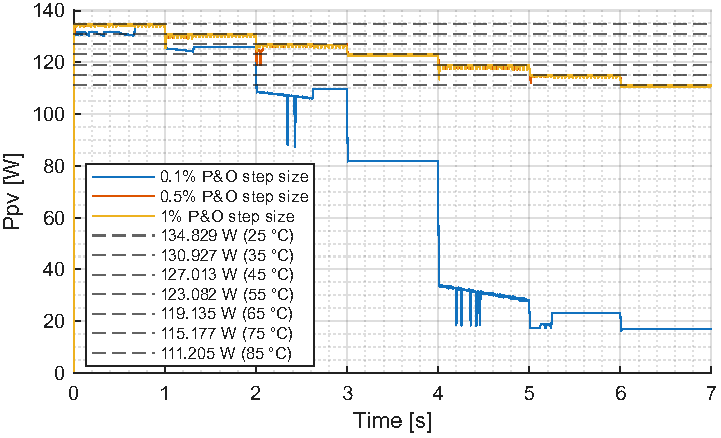
\includegraphics[width=\textwidth]{Images/Implementation/Tracking_speed_PEO_step2}
                \caption{Complete response.}
                \label{fig:peo_step_complete}
            \end{subfigure}
            \hfill
            \begin{subfigure}[b]{0.49\textwidth}
                \centering
                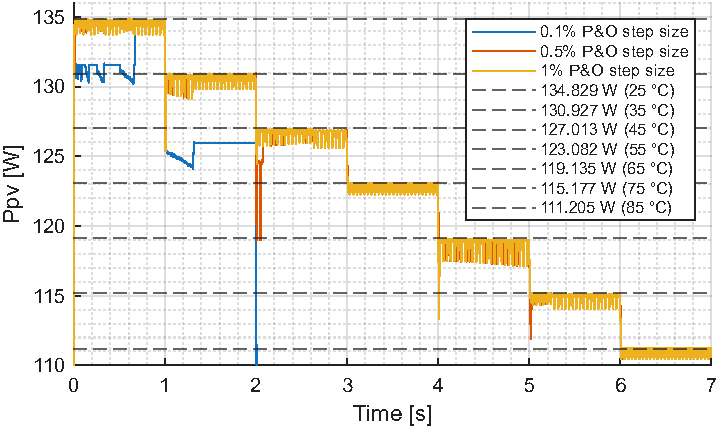
\includegraphics[width=\textwidth]{Images/Implementation/Tracking_speed_PEO_step.pdf}
                \caption{Zoomed view.}
                \label{fig:peo_step_zoom}
            \end{subfigure}

            \caption{Power response for different \ac{peo} step sizes during a temperature variation of $10~^\circ\mathrm{C/s}$.}
            \label{fig:peo_step_comparison}
        \end{figure}

        The analysis was then extended to more severe operating-point variations. For a temperature step from $25~^\circ\mathrm{C}$ to $85~^\circ\mathrm{C}$ (Figure~\ref{fig:big_temp_step}), the $0.5\%$ step, which had performed well previously, required about $1~\mathrm{s}$ to reach within $5\%$ of the \ac{mpp}. This meets the $1~\mathrm{s}$ limit but not the typical $0.5~\mathrm{s}$ target. The $1\%$ and $2\%$ steps were faster but oscillated more; a step between $0.5\%$ and $1\%$ is therefore the best compromise. Occasional stalls are caused by measurement noise and the \ac{peo} deadband and can be reduced by further tuning.

        A rapid irradiance variation was also simulated (Figure~\ref{fig:big_irr_step}). The \ac{mpp} is reached almost instantaneously for all step sizes, as expected, because the duty-cycle change is about three times smaller than in the temperature case.

        \begin{figure}[!ht]
            \centering
            \begin{minipage}[t]{0.48\textwidth}
                \centering
                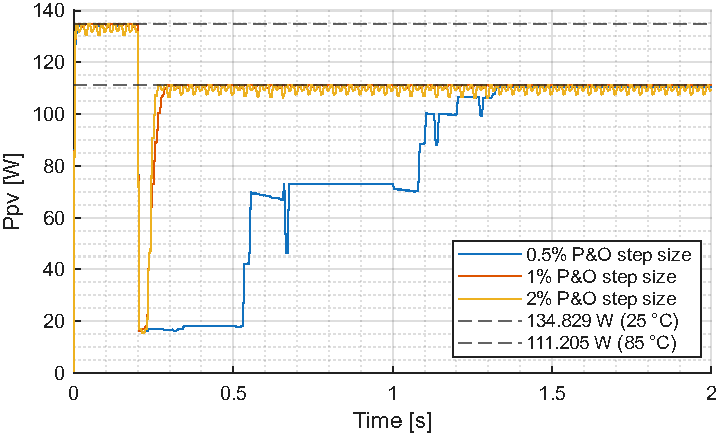
\includegraphics[width=\textwidth]{Images/Implementation/temp_step_PEOsteps.pdf}
                \caption{Power response for different \ac{peo} step sizes during a temperature variation from $25~^\circ\mathrm{C}$ to $85~^\circ\mathrm{C}$.}
                \label{fig:big_temp_step}
            \end{minipage}
            \hfill
            \begin{minipage}[t]{0.48\textwidth}
                \centering
                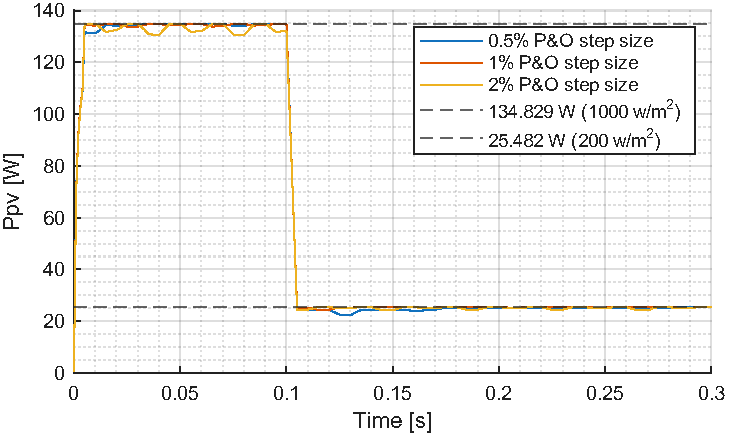
\includegraphics[width=\textwidth]{Images/Implementation/Irr_step_PEOsteps.pdf}
                \caption{Power response for different \ac{peo} step sizes during an irradiance variation from $1000~\mathrm{W/m}^2$ to $200~\mathrm{W/m}^2$.}
                \label{fig:big_irr_step}
            \end{minipage}
        \end{figure}